\section{Durchführung}
\label{sec:Durchführung}
Bei diesem Versuch stehen drei verschiedene Ultraschallsonden mit $\SI{1}{\mega\hertz}$,
$\SI{2}{\mega\hertz}$ und $\SI{4}{\mega\hertz}$, sowie ein Computer mit einem geeigneten
Programm zur Datenverarbeitung zur Verfügung.

\subsection{Untersuchung eines Acrylblocks}
Im ersten Versuchsteil soll ein Acrylblock mit mehreren Bohrungen mittels
A-Scan untersucht werden. Dieser ist schematisch in Abbildung \ref{fig:block}
dargestellt
\begin{figure}[H]
  \centering
  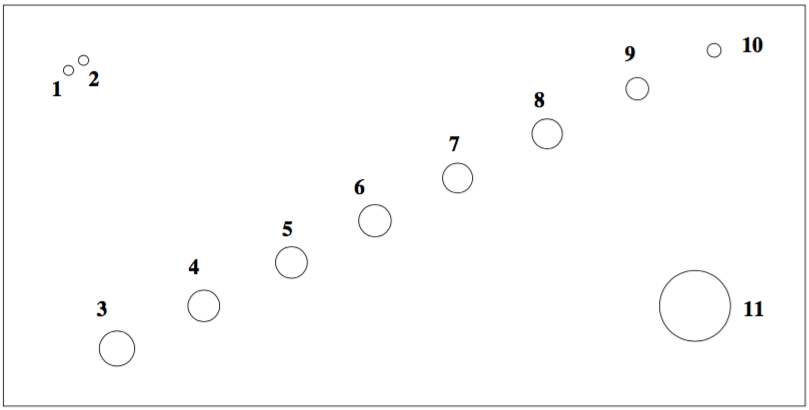
\includegraphics[height=6cm]{block.png}
  \caption{Schematische Darstellung des Acrylblocks}
  \label{fig:block}
  \cite{skript}
\end{figure}
Zunächst werden die Abmessungen des Blocks und der Bohrungen mit einer Schieblehre
vermessen. \\
Anschließend werden alle Bohrungen nochmal mit dem Impuls-Echo verfahren untersucht.
Dazu wird die $\SI{2}{\mega\hertz}$ Sonde verwendet, welche mit destilliertem Wasser
als Kontaktmittel von oben auf den Block angekoppelt wird. Am Computer ist die Einstellung
"A-Scan" zum wählen, zudem wird die Schallgeschwindigkeit $\SI{2730}{\meter\per\second}$
in Acryl aus der Vorbereitung eingestellt, um direkt die automatisch aus der Laufzeit berechneten
Tiefe der Störstelle ablesen zu können. Dabei wird die ganze Länge des Blocks einmal
mit der Sonde abgefahren, um alle Störstellen zu vermessen.
Analog wird noch einmal von der anderen Seite vorgegangen, indem der Block einmal
um 180° gedreht wird und die Messung wiederholt wird.

\subsection{Untersuchung des Auflösungsvermögens}
Um das Auflösungsvermögen der Sonden zu vergleichen, werden die beiden Bohrungen 1 und 2,
welche, wie in Abbildung \ref{fig:block} zu sehen ist, besonders eng beieinander liegen,
zusätzlich mit der $\SI{1}{\mega\hertz}$ Sonde untersucht, wobei die Graphiken
der beiden Messungen mit den zwei unterschiedlichen Sonden abgespeichert werden.

\subsection{Untersuchung des Acrylblocks mit dem B-Scan}
Der Acrylblock aus dem ersten Versuchsteil soll nun zusätzlich mit dem B-Scan untersucht werden.
Dazu wird am Computer die Darstellung "B-Scan" gewählt und die $\SI{2}{\mega\hertz}$ Sonde
erneut mit destilliertem Wasser angekoppelt. Nach Start der Messung wird mit der Sonde
dann mit möglichst konstanter und langsamer Geschwindigkeit die gesamte Länge des
Blocks abgefahren und die Graphik abgespeichert. Die Messung wird anschließend von
der anderen Seite wiederholt.

\subsection{Untersuchung eines Herzmodells mit dem TM-Scan}
Im letzten Teil des Versuches soll ein einfaches Herzmodell, bestehend aus
einem Doppelgefäß mit einer durch einen Gummiball auswölbbare Membran,
durch einen TM-Scan untersucht werden. Die Herzfrequenz und das Schlagvolumen kann hierbei
aus der typischen Kurve des "schlagenden" Herzens bestimmt werden.
Ist die Herzfrequenz $\nu_{\text{Herz}}$ bekannt lässt sich über das
enddiastolische Volumens (EDV) und des endsystolische Volumen (ESV) das Herzvolumen HZV
über
\begin{equation}
  \text{HZV}= (\text{EDS} - \text{HDV})\cdot \nu_{\text{Herz}}
\end{equation}
bestimmen. \\

Zur Messung wird das Herzmodell zunächst zu etwa einem Drittel mit destilliertem
Wasser gefühlt, woraufhin die $\SI{2}{\mega\hertz}$ Sonde so in eine Halterung
festgeschraubt wird, dass sie die Wasseroberfläche gerade berührt und durch einen
A-Scan die Membran sichtbar gemacht werden kann. Zu beachten ist, dass die eingestellte
Schallgeschwindigkeit von Acryl zu destilliertem Wasser gewechselt werden muss
($\text{c} = \SI{1480}{\meter\per\second}$ ), damit die Laufzeit korrekt zu Abständen
umgerechnet werden kann.
\\
Dann wird die Membran mit dem Gummiball leicht ausgewölbt, sodass die Sonde nicht zutief
in das Wasser eindringt und das Echo der Membran immer noch im A-Scan zu sehen ist.
Nun wird am Computer der "TM-Scan" eingestellt und nach dem Start der Messung die Membran
periodisch gewölbt, sodass die Herzfrequenz bzw. die Herzkurve aufgezeichnet wird.
Zudem wird der minimale und maximale Abstand zur Membran notiert.
Diese Graphik wird ebenfalls gespeichert.
